% Objectifs scientifiques et possibilités numériques

\subsection{Dialogue entre chercheurs et ingénieurs}
    \subsubsection{Concilier les besoins}
	L'intégration de traitements employant l'\ia à des projets de recherche en humanités implique une redéfinition des méthodes, pour adapter les pratiques des chercheurs aux nouveaux besoins soulevés par ces techniques. Dans la section précédentes, nous avons établi les nécessités et possibilités liées aux corpus de recherches, mais il est également crucial de prendre en compte les échanges entre les acteurs divers impliqués dans de telles initiatives. Les projets étudiés dans le cadre de ce mémoire -- notamment les projets \eida et \vhs -- présentent une architecture similaire en termes d'équipes impliquées : il est constitué une équipe d'historiens\footnote{Composée de chercheurs permanents, de chercheurs affiliés, de chercheurs postdoctorants et de doctorants.} menant des recherches sur les thèmes étudiés, travaillant en collaboration avec une équipe de chercheurs en vision artificielle\footnote{Dans les deux cas cités, il s'agit de l'équipe dirigée par Mathieu Aubry, appartenant au groupe de recherche \imagine.}. Les équipes d'histoire des sciences comptent, dans le cas de \vhs et \eida, un ou plusieurs ingénieurs, chargés de développement spécifiques et d'établir la communication avec les équipes de vision.
	
	Les deux équipes de recherche impliquées dans les projets font ainsi face à des besoins variés, qui ne sont pas nécessairement alignés. La communication établie entre ces deux pôles permet de clarifier les besoins en termes de traitement des sources historiques, par opposition aux besoins en termes de techniques, et particulièrement de définir les limites de ces méthodes et techniques numériques appliquées à l'histoire. Il se dessine alors une tension entre les attentes vis-à-vis des modèles de vision, et les possibilités réelles de la technique, qu'il est crucial de prendre en compte pour le développement d'outils à la fois performants et pertinents.
    
    \subsubsection{Utilité pour le \ml et intérêt historique}
	Ces tensions entre les besoins se manifestent dès les premières étapes de développement d'un modèle de vision artificielle : dans le cas du projet \eida, porté sur la détection de diagrammes dans les manuscrits, la confrontation entre l'aspect binaire de la détection et les nuances que doivent présenter l'approche historique se présente dès l'étape de constitution d'un premier jeu de données d'entraînement. En effet, cet aspect binaire du modèle, qui s'appuie sur l'opposition entre ce qui est un diagramme et ce qui n'en est pas un -- et plus largement, ce qui est une objet à détecter et ce qui n'en est pas un -- ne peut prendre en compte les cas limites qui se présentent systématiquement avec des sources historiques provenant d'un corpus aussi large. Se pose ainsi la question de la conciliation de ces deux exigences visiblement opposées : il est nécessaire de décider, par une discussion entre l'équipe de vision artificielle et l'équipe d'histoire des sciences, de ce qui est bel et bien un diagramme, selon les possibilités techniques et les besoins historiques.
	
	Une distinction se crée entre les pratiques utiles pour le \dl et les éléments intéressants pour les historiens. L'objectif, pour les deux équipes, est en effet de construire un outil utile aux résultats exploitables ; les projets ont donc pour devoir de prendre en compte ces besoins divergents, et d'établir un juste milieu entre les possibilités offertes et les objectifs initiaux. 
	
	Ainsi, dans cette situation, un équilibre est défini entre performances du modèle et pertinence historique, en prenant en compte le fait qu'il existe, après la détection, une intervention humaine : aucune solution n'étant pleinement satisfaisante, il convient de décider de celle qui permet de concilier les possibilités techniques et les objectifs scientifiques, afin de créer un outil qui produit des données exploitables, et qui automatise de manière pertinente le traitement des sources. Dans cette démarche, il est nécessaire de donner un cadre strict aux pratiques pour assurer une uniformisation des données, premier critère pour le développement d'outils numériques efficaces aux résultats cohérents.
    
\subsection{Définir les pratiques}
    \subsubsection{Traiter les cas limites}
	Il existe autant de manière de gérer ces situations qu'il existe de projet : les pratiques sont à définir en accord avec les besoins de chaque projet, sans qu'il n'existe de solution universelle. Les normes à appliquer sont à établir par un dialogue prenant en compte les ambitions techniques et scientifiques de chaque projet, ainsi que les spécificités des sources étudiées, qui présenteront des caractéristiques spécifiques propres à chaque corpus.
	
	En amont de la constitution du jeu de données pour l'entraînement du modèle de détection des diagrammes astronomiques du projet \eida, cette discussion entre l'équipe de l'Observatoire et celle du laboratoire \imagine a mené à la décision d'annoter tout type de diagramme, ainsi que les illustrations retrouvées dans les manuscrits, même lorsqu'elles ne correspondent pas aux objets recherchés. En effet, l'exclusion d'illustrations telles que les miniatures dans les données d'entraînement -- même si ces dernières ne correspondent pas aux objectifs scientifiques du projet -- pourrait produire un modèle aux détections lacunaires. La solution choisie l'a été en prenant en considération le fait qu'il est plus aisé pour un historien qui analyserait les images détectées d'exclure les illustrations qui ne sont pas des diagrammes, plutôt que de rechercher dans la numérisation des diagrammes manqués par un modèle aux performances insatisfaisantes.
	
	La création d'un premier jeu de données pour l'entraînement d'un modèle dédié à la détection des illustrations dans le corpus de \vhs a permis de mettre en lumière un certain nombre de cas limites, ou \textit{edge cases}, qui correspondent techniquement aux pratiques d'annotation définies par le projet, mais qui néanmoins impacteraient négativement les performances du modèle. Ainsi, nous voyons dans les annotations réalisées par les chercheurs de \vhs des pratiques à modifier (fig. \ref{fig:edge_cases_vhs}). Dans le premier cas, toutes les illustrations de la page n'ont pas été annotées : seule l'image principale de la planche zoologique est annotée comme un objet à détecter, tandis que les plus petites images sont délaissées. Comme mentionné précédemment, l'aspect manichéen de la détection par vision artificielle ne permet pas de hiérarchiser ainsi les images considérées intéressantes pour la recherche, et celles qui ne le sont pas, il est donc nécessaire d'annoter l'ensemble des illustrations pour ne pas impacter négativement les performances du modèle, et risquer une détection lacunaire. Dans les deuxième et troisième cas, les images annotées n'auraient pas dû l'être, car si la mauvaise qualité de la numérisation ou l'aspect fragmenté du document n'empêche pas un observateur humain d'identifier les illustrations comme telles, la compréhension de l'existence des parts manquantes de l'image tient de l'interprétation, et ne peut donc être attendue d'un modèle de vision artificielle\footnote{Elle pourrait l'être de la part d'un modèle entraîné sur un volume important de données, qu'il n'est pas envisageable de réunir à l'échelle d'un projet de recherche en histoire tel que \vhs.}. L'annotation de ce type d'objets pour l'entraînement du modèle risquerait ainsi d'altérer ses performances, en le poussant à détecter comme des illustrations des éléments qui n'en seraient pas.

	\begin{figure}[h]
		\begin{subfigure}{0.37\linewidth}
			\centering
			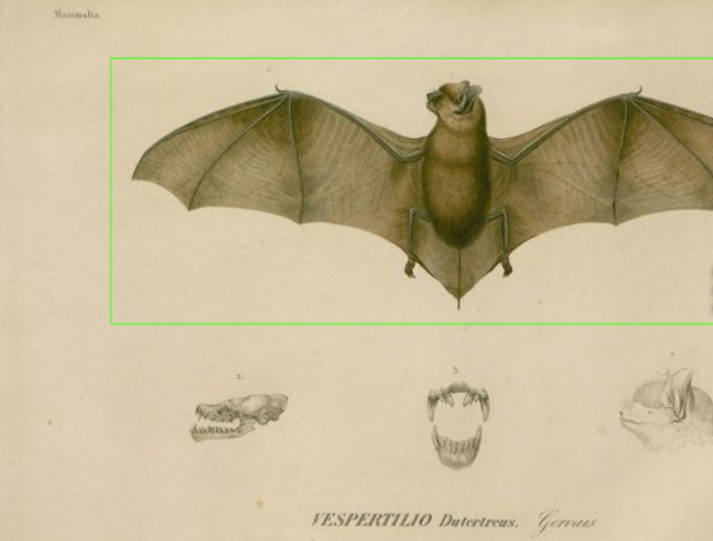
\includegraphics[height=4.5cm]{images/vhs_edge_case1.png}
			\subcaption{Annotation incomplète des illustrations}
		\end{subfigure}
		\hspace{1pt}
		\begin{subfigure}{0.30\linewidth}
			\centering
			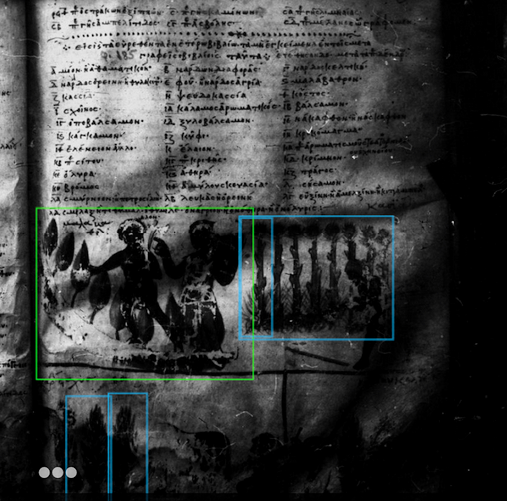
\includegraphics[height=4.5cm]{images/vhs_edge_case2.png}
			\subcaption{Annotation d'un document mal numérisé}
		\end{subfigure}
		\hspace{1pt}
		\begin{subfigure}{0.25\linewidth}
			\centering
			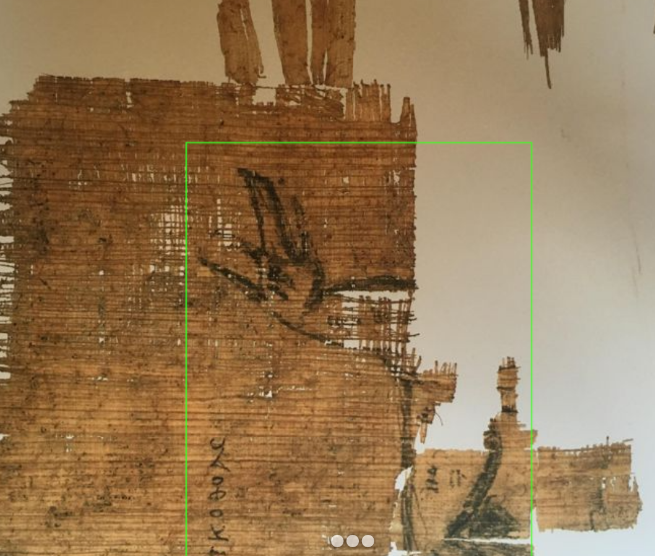
\includegraphics[height=4.5cm]{images/vhs_edge_case3.png}
			\subcaption{Annotation d'un document lacunaire}
		\end{subfigure}
		\caption{Cas limites rencontrés lors de l'annotation des images du projet \vhs}
		\label{fig:edge_cases_vhs}
	\end{figure}

	Ces décisions quant à l'annotation sont ainsi prises suite à un dialogue entre les équipes de chercheurs en vision et d'historiens, pour trouver un juste équilibre entre attentes et possibilités réelles. Des choix sont faits pour tirer parti des méthodes de vision artificielle, tout en acceptant que leurs résultats ne seront jamais identiques à ceux d'un travail manuel\footnote{De plus, un travail automatique présente des résultats uniformes et prévisibles, alors que les choix faits par des chercheurs varient selon les pratiques de chacun.} : les décisions doivent ainsi être prises pour exploiter de manière pertinentes ces techniques. Les pratiques définies par ces discussions entre les équipes mènent à des normes d'annotation : des spécifications sont alors rédigées pour les établir, et s'assurer de leur application uniforme, pour la création de données cohérentes.

    \subsubsection{Guides des pratiques : établir les normes}
	Pour s'assurer de l'application uniforme des normes d'annotation, il est de bonne pratique de rédiger une documentation à destination des chercheurs, à laquelle chacun peut se référer lors des étapes de création des données d'entraînement, qui constituent en elles-mêmes un travail considéré comme travail de recherche, puisqu'il requiert une connaissance et une compréhension des sources. Ainsi, les données produites suivent les mêmes règles, et cette cohérence assure une uniformité de jeu de données fourni au modèle de vision : cette uniformité permet, si une nouvelle étape d'entraînement est nécessaire, de corriger plus facilement les choix ayant mené à des résultats non-satisfaisants.
	
	Les chercheurs du projet \eida se sont vus fournir un \textit{Annotation Tutorial} en anglais, rédigé par Ségolène Albouy, cheffe de projet numérique, et Jil Le Bois, stagiaire de licence. Cette documentation fait suite à la mise en place d'une chaîne de traitement automatique des sources déposées par les chercheurs sur l'application du programme, qui produit une première détection que les chercheurs ont ensuite pour devoir de corriger. Le tutoriel qui a été communiqué contient des explications sur l'annotation dans l'application, avec un pas-à-pas détaillant chaque étape de ce travail, ainsi qu'une liste de cas pratiques établie en communication avec les historiens et l'équipe du laboratoire \imagine.
	
	Les cas pratiques établis répondent -- le plus souvent -- à des questions posées par les historiens à l'équipe d'ingénierie à l'occasion d'ateliers ou de séminaires, qui permettent de souligner au préalable les possibles doutes qui seront rencontrés lors de l'annotation. L'\textit{Annotation Tutorial} permet de garder trace de ces questionnements, et d'y apporter une réponse dont l'application sera systématique. La production de cette documentation, dont la responsabilité incombe aux ingénieurs d'étude, en tant que vecteurs de la communication entre les équipes d'histoire et de vision, pour donner à chaque parti impliqué la possibilité de se référer à un document qui rappelle les décisions prises. Cette possibilité de se référer à un document exhaustif est importante pour les étapes d'annotation, puisqu'elle garantit des données uniformes, mais aussi lors des étapes postérieures, notamment si d'autres entraînements sont nécessaires pour affiner les performances du modèle.
